\section{Site and Infrastructure}
\label{chap:Site}

\subsection{Site requirements and characterisation}
% author J.Harms
\label{SiteReq}
The achievable detector sensitivity and duty cycle, infrastructure lifetime, and its construction cost depend strongly on the characteristics of the ET site. This concerns underground parameters such as rock quality, groundwater, and site stability, but also surface parameters such as remoteness of the site, accessibility, and connection to existing infrastructure including public utility. In addition, socio-economic criteria must be considered for a big infrastructure like the Einstein Telescope, and it is important to understand and respect the interest of the local population. 

The achievable detector sensitivity, duty cycle and infrastructure lifetime are of prime interest to the science community. The impact of environmental noise on detector sensitivity is discussed in Section \ref{sec:envnoise}. The duty cycle of a detector also depends on its environment since regional earthquakes, but potentially also major storms, railroad traffic and other anthropogenic sources can produce enough ground motion to make a continuous operation of the detector challenging or impossible. In terms of ET's immediate science return, site parameters affecting the sensitivity of the detector are most important, but infrastructure lifetime determines how many cycles of major detector upgrades leading to sensitivity improvements one will be able to realize, which means that infrastructure lifetime plays an equally important role. 

The lifetime of an underground infrastructure is above all influenced by groundwater conditions (hydrogeology) and geological stability. Water inflow into tunnels requires water-handling systems, which might act as underground sources of seismic noise. Water that is being moved to the surface typically must be considered waste and pass through a water-treatment plant. The presence of water in the tunnels increases the humidity of the tunnel air, which drives atmospheric corrosion potentially accelerated by the presence of certain elements in groundwater such as chloride, and of microbes, e.g., sulfate-reducing bacteria, leading to microbially induced corrosion. Air humidity is controlled by ventilation systems that may also act as sources of underground seismic noise. With time, drainage systems to prevent water inflow can deteriorate leading to water leaks and tunnel lining deformation, which means that monitoring and maintenance are necessary in aged tunnels. 

Geological conditions determine the site stability. The most stringent requirements on differential motion across the tunnels does not come from the tunnel construction itself, but from the hosted detector infrastructure. The vacuum pipe will be mounted as a series of modules welded at their interfaces. Stress on the welding lips needs to remain small over the infrastructure lifetime. For example, across the 15\,m modules used in the Virgo detector, only a few millimeters of integrated differential displacement is tolerable. Another requirement comes from the positioning of the optical axis inside the vacuum pipe, which means that one needs to impose a maximum differential displacement across the full tunnel length as well. Drilling of the tunnel through active shear zones must therefore be avoided, and subsidence should be limited by driving the excavation through high-quality rock, or by employing hydraulic pipe-alignment systems like in Virgo.

Characterization of the site will happen in two steps. A preliminary survey of both candidate sites is required for site selection, relying mostly on surface measurements and analyses, and on a collection of already available site data. A few boreholes are mandatory to have at least some information about groundwater conditions, local geology, and underground seismic spectra. This information will be used to obtain first construction-cost estimates and to predict eventual complications in tunnel construction and maintenance. Characterization of environmental noise over at least a year is important to make accurate noise predictions for ET. Generally, the impact of the candidate sites' environments on ET sensitivity and operation needs to be assessed and evaluated. Solutions need to be found for waste removal (rock from excavation and tunnel water), and local support needs to be secured for realizing the ET infrastructure and for preserving the site quality. Once the site is chosen, extensive borehole studies of the future ET site will be necessary for construction planning and for a detailed cost estimate. 

\subsection {Newtonian Noise and other Environmental Noise}
\label{sec:envnoise}
% Author:  Jan Harms
Several environmental factors can influence the sensitivity of a gravitational-wave detector. Most importantly, seismic fields produce ground vibration that needs to be filtered out by a seismic isolation system for the suspended test masses. Seismic fields also lead to perturbations of the gravity field, which produces another random force on the test masses. Detector noise produced by terrestrial gravity fluctuations is also known as Newtonian noise to distinguish it from the effect of gravitational waves, which are described by general relativity. Similarly, atmospheric gravity fluctuations from acoustic, temperature and humidity fields are sources of Newtonian noise. Acoustic fields also act as sources of vibration of detector structure together with seismic fields. Electromagnetic fluctuations can produce detector noise by coupling with magnetic components of the detector, or by inducing noise at connectors and in cables acting as antennas. Finally, cosmic rays might cause test-mass charging, which then leads to excess noise by altering the dynamics and thus impeding the performance of the seismic isolation system. 

None of these environmental factors can be neglected ad hoc in ET. It is likely that test-mass charging by cosmic rays will not play a role in ET, and possibly is not the dominant charging mechanism in surface detectors either, since the underground environment acts as a shield against cosmic rays. Newtonian noise from atmospheric fields is mitigated by constructing ET several hundred meters underground leaving only minor (but likely significant) contributions to Newtonian noise from acoustic fields in the caverns. The seismic isolation system will be designed with the goal to provide sufficient seismic isolation without depending significantly on properties of the seismic field. Electromagnetic fluctuations, either being produced by the detector electronics or associated with Schumann resonances, depend weakly on the site where the detector will be built leaving seismic Newtonian noise as the main site-selection criterion with respect to environmental noise. It is crucial though that the underground environment will not be perturbed by detector infrastructure like the cryogenic system, water pumps, ventilation, and other machinery required to operate the detector. Experience with the Japanese underground detector KAGRA will help to optimize the ET infrastructure design to avoid excess noise.

Only some contributions to seismic Newtonian noise decrease with increasing detector depth. The contributions suppressed underground are mostly associated with seismic surface waves. Contributions from so-called body waves, i.e., seismic waves able to propagate in all directions through Earth, depend weakly on detector depth. In other words, the body-wave contribution sets a lower limit to seismic Newtonian noise, which is reached when the detector is so deep that body waves dominate the local seismic field and surface contributions can be neglected. Underground levels of seismic displacement are therefore a strong site-selection criterion. Newtonian noise in ET from seismic surface waves can also be significant, even many 100\,m underground, depending on seismic speeds. However, while there is no known technology that could mitigate effectively Newtonian noise from body waves, surface waves could be easily monitored by seismometer arrays and the seismic data be used to subtract efficiently the associated Newtonian noise from ET data if necessary. 

\subsection{Tunnels and Caverns}
% author G.Losurdo, A Paoli
\label{Sec:TunnelsCaverns} 

The design of the underground infrastructure is based on a trade-off between the
cost of the realization and the fulfillment of several scientific requirements,
such as, the capability of hosting the 6 interferometers, the availability of free space, safety, 
etc. The main elements are: the tunnels, the caverns, the access routes. Important
works are also needed on surface, with the realization of buildings and roads.

The underground scheme consists of an equilateral triangle of an approximate side length of 11\,km. The access is granted in the form of an inclined access tunnel or a vertical shaft, which connects the caverns at the intersection points with the surface.
The access tunnels/shafts are the main points of access during construction and operation. Several caverns of various geometry are situated in the vicinity of the intersection points. An additionally lined borehole/service tunnel offside the crucial and vibrational sensitive cavern structure is foreseen for water management during operation.

\paragraph{Tunnels}

%The three 10\,km tunnels will be excavated by TBMs, producing an inner free
%diameter of 6.5\,m.  
Due to the length of the tunnels, a mechanised excavation method utilising Tunnel Boring Machines (TBMs) is considered for the design stage. It is envisaged to excavate the whole length of the tunnel in one stretch without further points of intermediate access.
%\todo{Add a mentioning of mini-caverns every now and then (say 1\,km) for gate valves and pumping stations}
The inner diameter will be 6.5\,m, needed to host 4 vacuum pipes, which must be straight to several\,cm (and not follow Earth's curvature). The outer diameter could vary in a range between 7.3\,m and 8.4\,m depending on the type of TBM excavation (shielded or open TBM) and consequently by the kind of lining of the excavated tunnel (segmental pre-cast or shotcrete lining). 
The concept of the shielded TBM type considers a continuous mining process with parallel installation of a segmental lining, which takes over the support of the rock mass. A single-layer segmental lining with all-rounded preformed elastomer gaskets would be used to control water inflow to the tunnel. Thus the thickness of the reinforced concrete segments is at least 30\,cm.
Contrary to a shielded TBM, the open TBM is based on applying shotcrete, steel ribs and rock bolts. As part of the excavation concept, rock mass grouting is considered, to decrease the overall inflow of groundwater to the tunnel, since the shotcrete support is more prone to water inflow.
The overall thickness of the shotcrete support layers is also of the order of 30\,cm thick consisting of two layers. Regardless of the straight direction demanded for the subsequent installation of the vacuum pipes in the tunnels, the TBM excavation implies an inherent meandering of the tunnel axis as a reaction to heterogeneous geological conditions while driving. 
%A predefined additional over-excavation should be considered, to avoid interference of the clearance profile of the tunnel with needed space the steel tubes, which is of the order of 10 cm for the open TBM, while 65 cm for the shielded one [TBD].
 \begin{figure}[tbh]
	\centering
		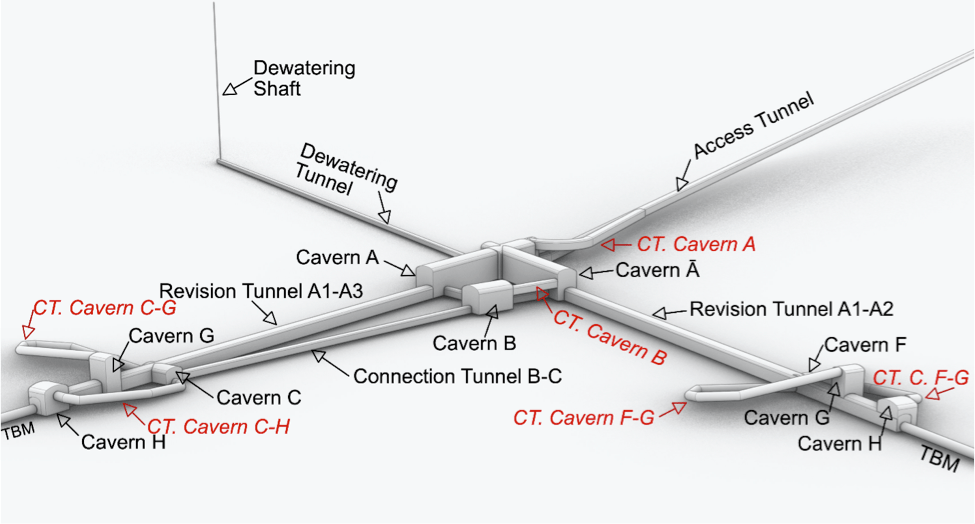
\includegraphics[width=0.9\textwidth]{Figures/ET_caverns.png}
	\caption{Sketch of the cavern layout of the ET in one corner of the
	triangle. 
	All labels in red refer to constructionally required galleries or tunnels.
	\label{fig:ET_caverns}}
\end{figure}

\paragraph{Caverns}

For each vertex of the triangle layout, “Cavern A” (see Figure~\ref{fig:ET_caverns}) indicates the main cavern structure of the underground laboratory and is formed by an intersection of two caverns with an identical layout at an angle of 60°, with lengths of about 190 m and 160 m.
The smaller cavern branch (Cross-Cavern A) includes a prolongation tunnel about 1 km long, hosting the Filter Cavity. 
Two identical connecting 465\,m long tunnels run in the prolongation of the branches of “Cavern A”. Each connecting tunnel contains a series of three caverns (Cavern C-F/G/H) at the transition to the TBM tunnel. The three caverns have a spacing of 35\,m in between them. 
%The distance between the caverns is mainly required from an operational point of view but will be also deemed to be adequate from a geomechanical perspective.
The “Cavern B” is located within the bisection line of the two branches of the “connecting tunnels”. It is linked to the two branches of the “Cavern A” and carries an additional connection tunnel to the Cavern C. 
%The Cavern C is situated 316 m offside the Cavern B and the connection tunnel will host the filter cavity reserved to the “calibration” of the interferometer [TBD].
The caverns and the connecting tunnel are of various shapes and will be excavated by drill and blast. The design foresees a horseshoe-shaped design of all cavern, tunnels and galleries. The shape of these caverns and tunnels might be redesigned to fit the geomechanical requirements.

\paragraph{Access}
    
The underground infrastructure can be accessed by elongated inclined tunnel ramps or large vertical shafts. The best option may strongly depend on the geography, geology and surface land use and will therefore be finalized after the choice of the site. 

Three construction methods are available: access by inclined elongated ramp; access by inclined helical ramp; access by vertical shaft.
An “inclined elongated ramp” equally to an “inclined helical ramp” connects the
surface with the cavern structure situated a few 100\,m below the ground surface. The length of the access tunnel is considered based an overall slope of max. 10\%. It is not required to drive the access tunnel as a straight line, any combination of the straight and curved section is possible.
The clearance profile of any inclined tunnel shall support all aspects of construction, mucking and ventilation. 

Daylighting shafts are the shortest connection of the surface to the underground structure. The vertical shaft is considered as the single line of access during construction and operation. Nevertheless, for the long-term service, changes to the shaft hauling system are necessary to comply with the demands of the laboratory.

The decision on the best type of access depends on a combination of ecological, logistical (connecting roads), geological/hydro-geological, safety and monetary aspects. 
Due to further site-dependent impact factors, currently only the monetary
aspects of the access have been analysed. 
%In any way from a constructional point of
%view, the inclined access tunnel is the most conservative layout. 
Both types of access can be accomplished with standard tunnelling equipment.
The shaft solution implies the utilisation of specialised equipment for shaft lowering, while the inclined access tunnel can be excavated with standard tunnelling equipment, as foreseen in any way for the excavation of the underground caverns.

\subsection{Roads and buildings}
% author G.Losurdo, A Paoli
\label{Sec:RoadsBuildings}

The construction of the ET facility will include all the surface technical and general buildings needed for the construction and operation of the research centre.
The surface buildings will be located mainly in correspondence of the access points to the underground infrastructure and consist of the following list, with the corresponding estimated volume at this stage of the project: laboratories for the construction and the installation, warehouses, clean rooms, mechanical and electrical workshops, control buildings, office buildings, technical buildings for plants, visitor centre, access buildings.
%TODO  [Volume per category to be added].

